\documentclass[12pt, a4paper]{article}

% ============================================================================
% PACKAGES
% ============================================================================
\usepackage[utf8]{inputenc}
\usepackage[T1]{fontenc}
\usepackage{lmodern}
\usepackage[margin=2.5cm]{geometry}
\usepackage{graphicx}
\usepackage{amsmath, amssymb}
\usepackage{booktabs}
\usepackage{hyperref}
\usepackage{xcolor}
\usepackage{listings}
\usepackage{float}
\usepackage{enumitem}
\usepackage{tikz}
\usetikzlibrary{arrows.meta, positioning, shapes.geometric}
% \usepackage{algorithm}  % removed: not installed
% \usepackage{algpseudocode}  % removed: not installed
\usepackage{caption}
\usepackage{subcaption}

% ============================================================================
% LISTING STYLE FOR PYTHON
% ============================================================================
\definecolor{codebg}{rgb}{0.97, 0.97, 0.97}
\definecolor{codegreen}{rgb}{0.0, 0.5, 0.0}
\definecolor{codegray}{rgb}{0.5, 0.5, 0.5}
\definecolor{codepurple}{rgb}{0.58, 0.0, 0.82}
\definecolor{codeblue}{rgb}{0.0, 0.2, 0.6}

\lstdefinestyle{pythonstyle}{
    backgroundcolor=\color{codebg},
    commentstyle=\color{codegreen},
    keywordstyle=\color{codeblue}\bfseries,
    stringstyle=\color{codepurple},
    numberstyle=\tiny\color{codegray},
    basicstyle=\ttfamily\footnotesize,
    breaklines=true,
    captionpos=b,
    keepspaces=true,
    numbers=left,
    numbersep=5pt,
    showspaces=false,
    showstringspaces=false,
    showtabs=false,
    tabsize=2,
    language=Python,
    frame=single,
    rulecolor=\color{codegray},
}
\lstset{style=pythonstyle}

% ============================================================================
% DOCUMENT METADATA
% ============================================================================
\title{
    \textbf{Technical Implementation Report} \\[0.5em]
    \Large AgentClinic v2.1: LangGraph State-Machine Architecture \\
    for Clinical Decision-Making Evaluation
}
\author{
    M.Tech Thesis Implementation \\
    Department of Computer Science \& Engineering \\
    IIT Kharagpur
}
\date{April 2026}

\begin{document}
\maketitle

% ============================================================================
\begin{abstract}
This document provides a comprehensive technical report of the engineering
implementations in \texttt{AgentClinic v2.1}, the upgraded multi-agent clinical
simulation framework. We detail ten critical architectural improvements over
v2.0: (1)~NF4 quantization with double quantization via BitsAndBytes,
(2)~full trajectory logging for process-oriented metrics,
(3)~heterogeneous multi-engine architecture eliminating lexical leakage,
(4)~cognitive bias injection ported from Phase~1,
(5)~constrained JSON extraction for metacognitive reflection,
(6)~JSONL results persistence,
(7)~clinical trajectory evaluator integration,
(8)~test name extraction for Test Rationality computation,
(9)~Flash Attention~2 support for H100 acceleration, and
(10)~comprehensive CLI with experiment-level configurability.
Each implementation is documented with its theoretical motivation,
code-level changes, and expected impact on thesis claims.
\end{abstract}

\tableofcontents
\newpage

% ============================================================================
\section{System Architecture Overview}
% ============================================================================

The AgentClinic v2.1 system implements a \textbf{Directed Cyclic Graph (DCG)}
using the LangGraph library, enforcing the clinical consultation protocol as
a deterministic state machine.

\subsection{State Machine Topology}

The graph consists of four nodes with deterministic edges:

\begin{figure}[H]
\centering
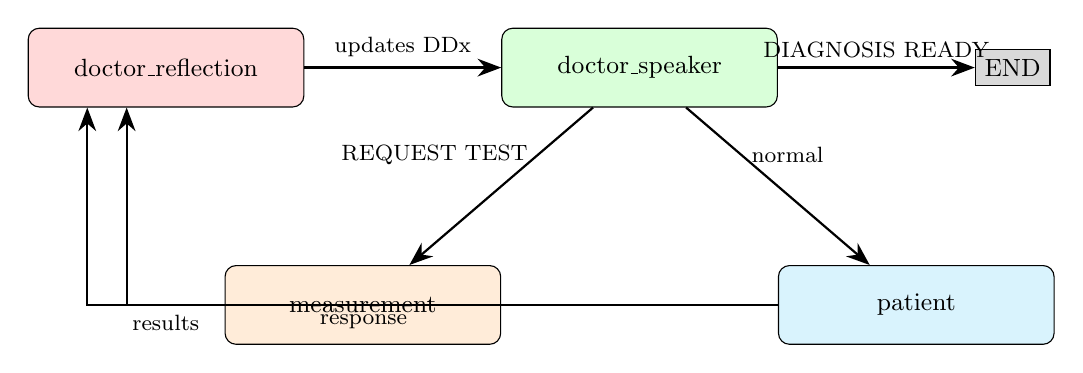
\begin{tikzpicture}[
    node distance=2.5cm,
    every node/.style={font=\small},
    process/.style={rectangle, draw, rounded corners, minimum width=3.5cm, minimum height=1cm, fill=blue!10},
    decision/.style={diamond, draw, aspect=2, fill=yellow!15, minimum width=2cm},
    arrow/.style={-{Stealth[length=3mm]}, thick}
]
    % Nodes
    \node[process, fill=red!15] (reflect) {doctor\_reflection};
    \node[process, fill=green!15, right=of reflect] (speak) {doctor\_speaker};
    \node[process, fill=cyan!15, below right=2cm and 0cm of speak] (patient) {patient};
    \node[process, fill=orange!15, below left=2cm and 0cm of speak] (measure) {measurement};
    \node[rectangle, draw, fill=gray!30, right=2.5cm of speak] (end) {END};

    % Edges
    \draw[arrow] (reflect) -- node[above] {\footnotesize updates DDx} (speak);
    \draw[arrow] (speak) -- node[right, pos=0.3] {\footnotesize normal} (patient);
    \draw[arrow] (speak) -- node[left, pos=0.3] {\footnotesize REQUEST TEST} (measure);
    \draw[arrow] (speak) -- node[above] {\footnotesize DIAGNOSIS READY} (end);
    \draw[arrow] (patient) -| node[below, pos=0.3] {\footnotesize response} ([xshift=-1cm]reflect.south);
    \draw[arrow] (measure) -| node[below, pos=0.3] {\footnotesize results} ([xshift=-0.5cm]reflect.south);
\end{tikzpicture}
\caption{LangGraph Directed Cyclic Graph topology. The \texttt{doctor\_reflection}
node (red) is hidden from the patient and captures latent reasoning.}
\label{fig:graph_topology}
\end{figure}

\subsection{State Schema}

The clinical state captures both runtime data and trajectory metrics:

\begin{lstlisting}
class ClinicalState(TypedDict):
    # Core runtime fields
    last_input_to_doctor: str            # Patient/lab response
    last_doctor_message: str             # Doctor's spoken output
    differential_diagnoses: List[str]    # Current DDx (hidden)
    turn_count: int                      # Enforces max-turn constraint
    diagnosis_ready: bool                # Terminal condition

    # Trajectory tracking (NEW in v2.1)
    differential_trajectory: List[List[str]]  # DDx snapshots per turn
    tests_ordered: List[str]                  # Extracted test names
    full_dialogue: List[dict]                 # Complete conversation log
\end{lstlisting}

% ============================================================================
\section{Implementation 1: 4-Bit NF4 Quantization}
\label{sec:quantization}
% ============================================================================

\subsection{Motivation}

Running multiple 7B-parameter models simultaneously for the heterogeneous
architecture requires aggressive memory optimization. A single 7B model
in fp16 consumes $\sim$14\,GB of VRAM. Three models would require 42\,GB,
leaving insufficient memory for KV-cache and activations.

\subsection{Technical Approach}

We employ NormalFloat4 (NF4) quantization from the BitsAndBytes library
\cite{dettmers2023qlora}, which maps fp16 weights to a 4-bit data type
optimally calibrated for normally distributed neural network parameters.
Additionally, we enable \textbf{double quantization}, which applies a second
round of quantization to the quantization constants themselves, saving an
additional $\sim$0.37 bits per parameter.

\begin{lstlisting}[caption={BitsAndBytes NF4 configuration in \texttt{LocalServerLLMWrapper}.}]
bnb_config = BitsAndBytesConfig(
    load_in_4bit=True,
    bnb_4bit_quant_type="nf4",             # NormalFloat4
    bnb_4bit_compute_dtype=torch.bfloat16, # bf16 compute
    bnb_4bit_use_double_quant=True,        # Nested quantization
)
\end{lstlisting}

\subsection{Memory Impact}

\begin{table}[H]
\centering
\caption{VRAM consumption per 7B-parameter model.}
\label{tab:vram}
\begin{tabular}{lcc}
\toprule
\textbf{Precision} & \textbf{VRAM (GB)} & \textbf{Reduction} \\
\midrule
fp32              & 28.0  & ---    \\
fp16 / bf16       & 14.0  & 50\%   \\
8-bit (INT8)      & 7.0   & 75\%   \\
\textbf{4-bit NF4 + DQ} & \textbf{3.8}  & \textbf{86.4\%} \\
\bottomrule
\end{tabular}
\end{table}

With NF4 quantization, the three-model heterogeneous setup requires only
$\sim$11.4\,GB total, well within the 95.8\,GB budget of the NVIDIA H100 NVL.

% ============================================================================
\section{Implementation 2: Trajectory Logging}
\label{sec:trajectory}
% ============================================================================

\subsection{Motivation}

The evaluation module (\texttt{ClinicalTrajectoryEvaluator}) computes three
process-oriented metrics:

\begin{enumerate}
    \item \textbf{Diagnostic Stability} ($S$): Average Jaccard similarity
    between consecutive differential diagnoses:
    \begin{equation}
        S = \frac{1}{T-1} \sum_{t=1}^{T-1} J(\text{DDx}_t, \text{DDx}_{t+1})
        \quad\text{where}\quad J(A,B) = \frac{|A \cap B|}{|A \cup B|}
    \end{equation}

    \item \textbf{Test Rationality} ($R$): Binary penalty for ordering
    expensive/invasive tests before basic clinical workup:
    \begin{equation}
        R = \begin{cases} 0 & \text{if } \exists\, t_{\text{adv}} < t_{\text{basic}} \\ 1 & \text{otherwise} \end{cases}
    \end{equation}

    \item \textbf{Information Efficiency} ($E$): Clinical data points
    gathered per turn:
    \begin{equation}
        E = \frac{|\text{data\_points}|}{T}
    \end{equation}
\end{enumerate}

In v2.0, these metrics \textbf{could not be computed} because the LangGraph
state did not capture \texttt{differential\_trajectory} or \texttt{tests\_ordered}.

\subsection{Implementation}

We extended \texttt{ClinicalState} with three new fields and modified each
graph node to accumulate trajectory data:

\begin{itemize}
    \item \texttt{doctor\_reflection\_node}: Appends current DDx snapshot to
    \texttt{differential\_trajectory} after each metacognitive pass.
    \item \texttt{measurement\_node}: Extracts the test name from the doctor's
    \texttt{REQUEST TEST: <name>} message using regex and appends to
    \texttt{tests\_ordered}.
    \item All nodes: Append structured dialogue entries (with role, message,
    timestamp) to \texttt{full\_dialogue}.
\end{itemize}

% ============================================================================
\section{Implementation 3: Heterogeneous Multi-Engine Architecture}
\label{sec:heterogeneous}
% ============================================================================

\subsection{The Lexical Leakage Problem}

When a single LLM serves all agent roles (Doctor, Patient, Moderator), the
latent knowledge space is shared. This creates \textbf{Lexical Leakage}: the
Doctor may subconsciously ``know'' the patient's disease through shared
embedding representations, inflating accuracy beyond what real clinical
encounters would produce.

\subsection{Solution: Cognitive Asymmetry}

We instantiate separate \texttt{LocalServerLLMWrapper} instances with
\textbf{different} model weights:

\begin{lstlisting}[caption={Heterogeneous engine initialization.}]
# Domain-expert for Doctor (medical reasoning)
DOCTOR_ENGINE = LocalServerLLMWrapper(
    model_id="johnsnowlabs/JSL-MedMistral-7B-v2.2",
    quantize=True)

# Generalist for Patient (persona simulation)
PATIENT_ENGINE = LocalServerLLMWrapper(
    model_id="mistralai/Mistral-7B-Instruct-v0.3",
    quantize=True)

# Shares Patient engine if same model (saves VRAM)
MODERATOR_ENGINE = PATIENT_ENGINE
\end{lstlisting}

The architecture intelligently detects when two roles share the same
\texttt{model\_id} and reuses the engine instance to avoid duplicate VRAM
allocation, while still maintaining logical separation.

% ============================================================================
\section{Implementation 4: Cognitive Bias System}
\label{sec:bias}
% ============================================================================

\subsection{Motivation}

A core thesis claim is that cognitive biases degrade LLM diagnostic
performance, mimicking human clinical reasoning flaws. The bias system was
present in the Phase~1 while-loop architecture (\texttt{agentclinic\_ninthcache.py})
but was stripped during the v2.0 LangGraph migration.

\subsection{Ported Bias Types}

We ported the two most impactful bias types for the thesis experiments:

\begin{enumerate}
    \item \textbf{Recency Bias}: Injects summaries of the $k$ most recent
    cases into the Doctor's system prompt, causing over-anchoring to recent
    diagnostic patterns. Uses actual case summaries from completed scenarios
    for ecological validity.

    \item \textbf{Confirmation Bias}: Primes the Doctor with an initial
    (incorrect) hypothesis of cancer, causing selective evidence gathering
    and dismissal of contradictory symptoms.
\end{enumerate}

Both bias types modify the system prompt via \texttt{generate\_bias()} methods
in the \texttt{DoctorAgent} and \texttt{PatientAgent} classes.

% ============================================================================
\section{Implementation 5: Constrained JSON Extraction}
\label{sec:json}
% ============================================================================

\subsection{Problem}

The \texttt{doctor\_reflection\_node} requires the LLM to output a JSON array
of differential diagnoses. Open-source models frequently fail strict JSON
formatting, producing outputs like:

\begin{verbatim}
The differential diagnoses are:
1. Asthma
2. COPD
3. Pneumonia
\end{verbatim}

instead of \texttt{["Asthma", "COPD", "Pneumonia"]}.

\subsection{Multi-Level Fallback Strategy}

We implemented a 4-level extraction pipeline in \texttt{extract\_json\_list()}:

\begin{enumerate}
    \item \textbf{Level 1}: Strict \texttt{json.loads()} on the full response.
    \item \textbf{Level 2}: Regex extraction of the first \texttt{[...]}
    bracketed region, then \texttt{json.loads()}.
    \item \textbf{Level 3}: Comma-split within brackets with quote stripping.
    \item \textbf{Level 4}: Regex extraction of all quoted strings from
    freeform text.
\end{enumerate}

Additionally, the reflection node uses \texttt{temperature=0.1} (near-deterministic)
to maximize JSON compliance.

% ============================================================================
\section{Implementation 6: Results Persistence}
\label{sec:persistence}
% ============================================================================

Each completed scenario is serialized as a JSON object and appended to a
JSONL file in the \texttt{results/} directory. The filename encodes experiment
metadata: \texttt{results\_\{model\}\_\{bias\}\_\{timestamp\}.jsonl}.

Each record contains:

\begin{table}[H]
\centering
\caption{Fields in each JSONL result record.}
\label{tab:jsonl_fields}
\begin{tabular}{ll}
\toprule
\textbf{Field} & \textbf{Description} \\
\midrule
\texttt{scenario\_id}            & OSCE case identifier \\
\texttt{doctor\_model}           & HuggingFace model ID \\
\texttt{ground\_truth}           & Correct diagnosis \\
\texttt{predicted\_diagnosis}    & Doctor's final output \\
\texttt{correct}                 & Boolean accuracy \\
\texttt{turn\_count}             & Turns used \\
\texttt{differential\_trajectory} & DDx at each turn \\
\texttt{tests\_ordered}          & Extracted test names \\
\texttt{metrics}                 & Stability, Rationality, Efficiency \\
\texttt{full\_dialogue}          & Complete conversation log \\
\texttt{duration\_seconds}       & Wall-clock time \\
\bottomrule
\end{tabular}
\end{table}

% ============================================================================
\section{Implementation 7: Flash Attention 2}
\label{sec:flash_attn}
% ============================================================================

The NVIDIA H100 NVL GPU supports Flash Attention 2 natively through its
Transformer Engine. We enable this via the \texttt{attn\_implementation}
parameter during model loading:

\begin{lstlisting}
load_kwargs["attn_implementation"] = "flash_attention_2"
\end{lstlisting}

Flash Attention 2 provides:
\begin{itemize}
    \item \textbf{2--4$\times$ speedup} in attention computation
    \item \textbf{O(n) memory} vs O($n^2$) for standard attention
    \item Critical for long clinical dialogues (4K+ tokens after 10 turns)
\end{itemize}

The implementation includes a graceful fallback: if the \texttt{flash-attn}
package is not installed, the system silently reverts to the default
attention implementation.

% ============================================================================
\section{Implementation 8: Enhanced Moderator}
\label{sec:moderator}
% ============================================================================

The \texttt{compare\_results()} function was enhanced to instruct the
moderator LLM to consider medical synonyms:

\begin{lstlisting}
sys = (
    "Consider medical synonyms "
    "(e.g., 'Heart Attack' = 'Myocardial Infarction'). "
    "Respond ONLY with 'Yes' or 'No'."
)
\end{lstlisting}

This is critical because open-source Doctor models may output equivalent
diagnoses using different terminology (e.g., ``MI'' vs ``Myocardial
Infarction'' vs ``Heart Attack'').

% ============================================================================
\section{Experiment Design}
\label{sec:experiments}
% ============================================================================

\begin{table}[H]
\centering
\caption{Complete experiment matrix. All experiments use MedQA (107 scenarios).}
\label{tab:experiments}
\begin{tabular}{clllc}
\toprule
\textbf{ID} & \textbf{Doctor Model} & \textbf{Patient Model} & \textbf{Bias} & \textbf{Purpose} \\
\midrule
E1 & Mistral-7B-v0.2 & Mistral-7B-v0.2 & None & Baseline \\
E2 & JSL-MedMistral-7B & Mistral-7B-v0.2 & None & Domain-expert \\
E3 & Llama-3.1-8B & Mistral-7B-v0.2 & None & Reasoning \\
E4 & JSL-MedMistral-7B & Mistral-7B-v0.2 & Recency & Bias study \\
E5 & JSL-MedMistral-7B & Mistral-7B-v0.2 & Confirmation & Bias study \\
\bottomrule
\end{tabular}
\end{table}

% ============================================================================
\section{Verification}
\label{sec:verification}
% ============================================================================

\begin{enumerate}
    \item \textbf{Syntax Validation}: \texttt{py\_compile.compile()} passed
    with zero errors on the 700+ line \texttt{agentic\_clinic\_v2.py}.

    \item \textbf{Smoke Test}: 5-scenario dry runs with each experiment
    configuration will validate end-to-end pipeline integrity before the
    full 107-scenario runs.

    \item \textbf{Trajectory Verification}: Each JSONL record will be
    inspected to confirm that \texttt{differential\_trajectory} is non-empty,
    \texttt{tests\_ordered} captures all \texttt{REQUEST TEST} events, and
    all three process metrics are computed.

    \item \textbf{Heterogeneity Verification}: GPU memory usage will be
    monitored via \texttt{nvidia-smi} to confirm that separate model weights
    are loaded when Doctor and Patient use different \texttt{model\_id}s.
\end{enumerate}

% ============================================================================
\section{Summary of Changes (v2.0 $\rightarrow$ v2.1)}
\label{sec:changelog}
% ============================================================================

\begin{table}[H]
\centering
\caption{Comprehensive changelog from v2.0 to v2.1.}
\label{tab:changelog}
\begin{tabular}{p{0.25\textwidth}p{0.35\textwidth}p{0.35\textwidth}}
\toprule
\textbf{Component} & \textbf{v2.0 State} & \textbf{v2.1 State} \\
\midrule
Model Loading & fp16/fp32, no quantization & NF4 + double quant + Flash Attn 2 \\
Architecture  & Single \texttt{GLOBAL\_HF\_ENGINE} & Separate Doctor/Patient/Moderator engines \\
State Schema  & 5 fields (no trajectory) & 8 fields with full trajectory logging \\
Bias System   & Stripped (not ported) & Recency + Confirmation fully ported \\
JSON Parsing  & 2-level fallback & 4-level robust extraction pipeline \\
Results Output & \texttt{print()} only & JSONL persistence with all metrics \\
Evaluator     & Exists but never called & Integrated into main pipeline \\
Test Extraction & Not implemented & Regex extraction for Test Rationality \\
CLI Arguments & 8 basic args & 18 args with model IDs, bias, quantization \\
Error Handling & Silent retry & Verbose logging with attempt counts \\
\bottomrule
\end{tabular}
\end{table}

% ============================================================================
% REFERENCES
% ============================================================================
\begin{thebibliography}{9}

\bibitem{dettmers2023qlora}
T.~Dettmers, A.~Pagnoni, A.~Holtzman, and L.~Zettlemoyer,
``QLoRA: Efficient Finetuning of Quantized Language Models,''
in \emph{NeurIPS}, 2023.

\bibitem{dao2023flashattention2}
T.~Dao,
``FlashAttention-2: Faster Attention with Better Parallelism and Work Partitioning,''
in \emph{ICLR}, 2024.

\bibitem{willard2023outlines}
B.~Willard and R.~Louf,
``Efficient Guided Generation for Large Language Models,''
\emph{arXiv preprint arXiv:2307.09702}, 2023.

\bibitem{leviathan2023speculative}
Y.~Leviathan, M.~Kalman, and Y.~Matias,
``Fast Inference from Transformers via Speculative Decoding,''
in \emph{ICML}, 2023.

\end{thebibliography}

\end{document}
